In this part the additional closure plots are shown.


% ttbar MHT closure iso reco acc
\begin{figure}[tbhn]
\begin{center}
\begin{tabular}{cc}
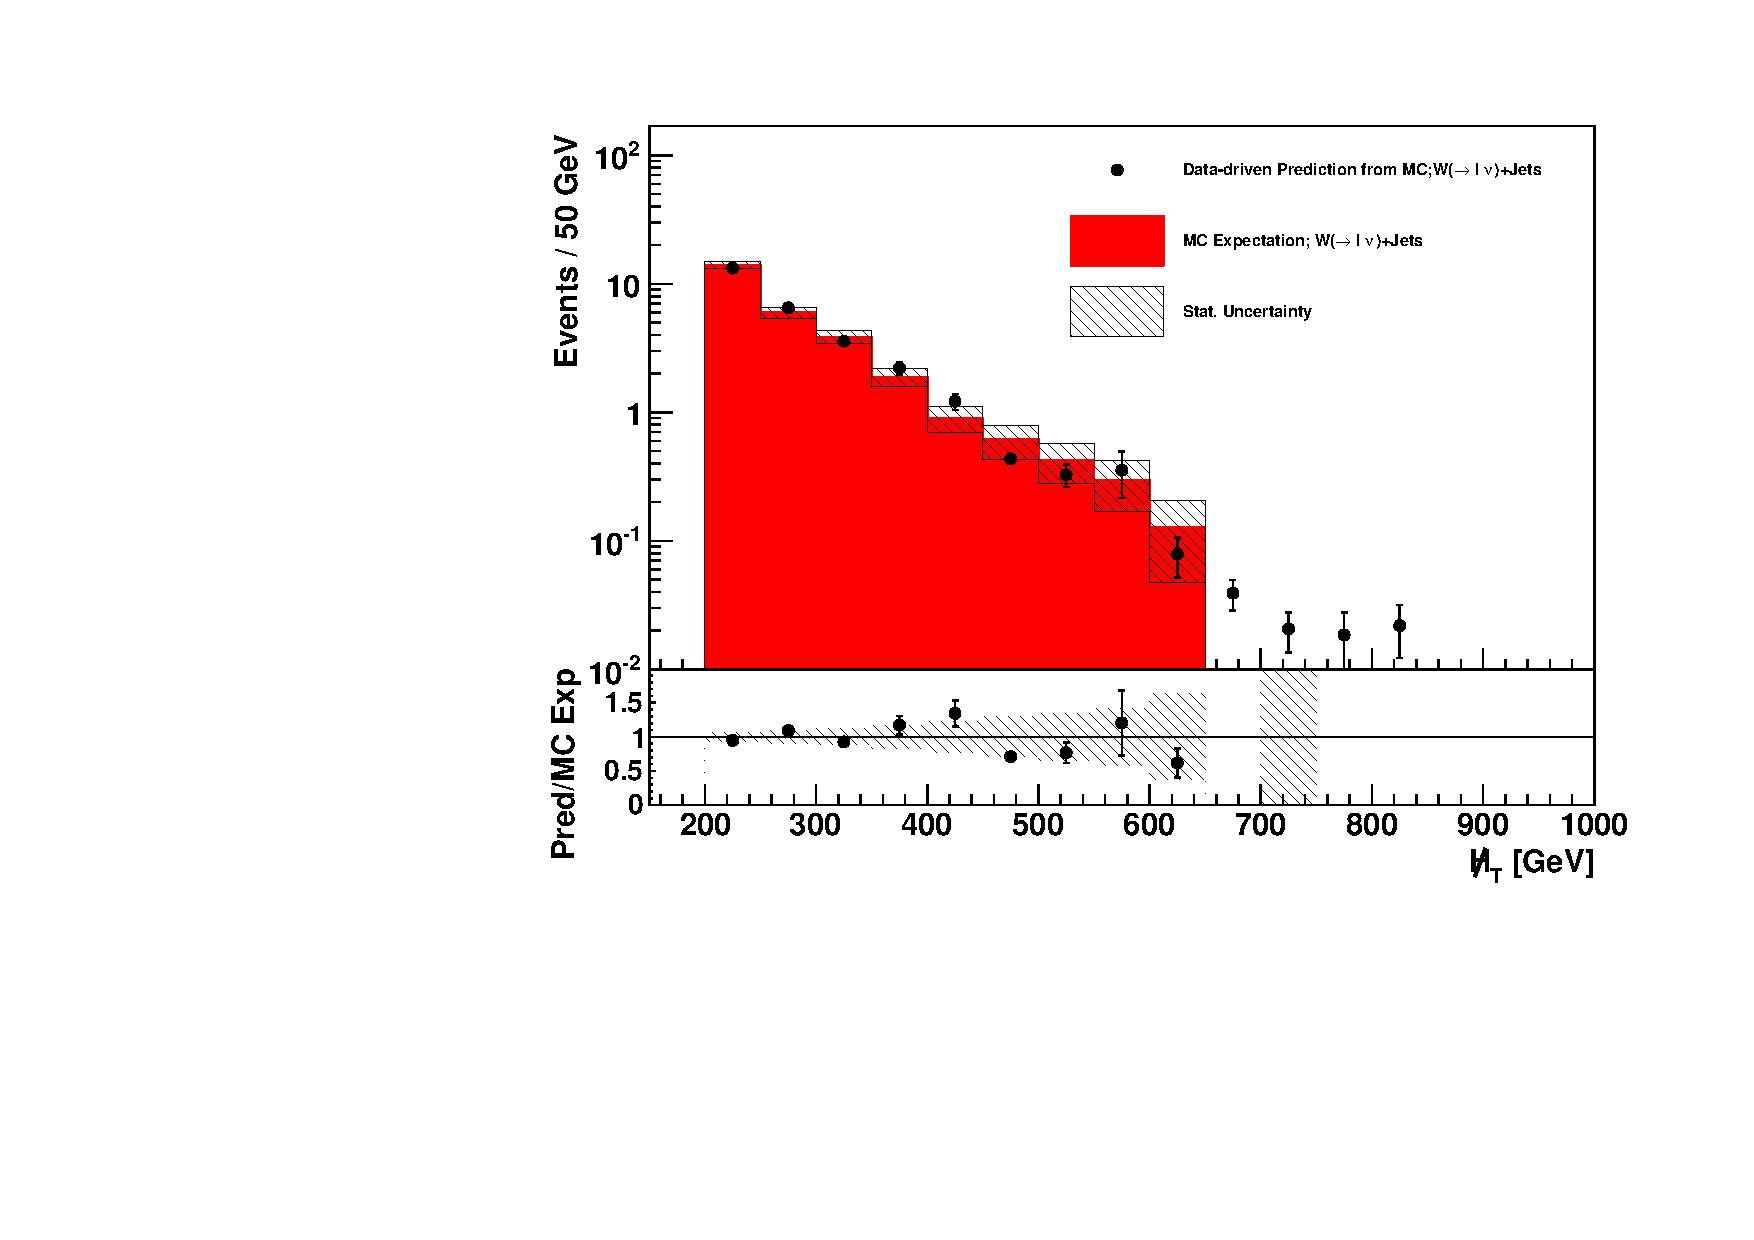
\includegraphics[width=0.45\textwidth]{lostlepton/plots/closure/MHTwIsoMu.pdf} 
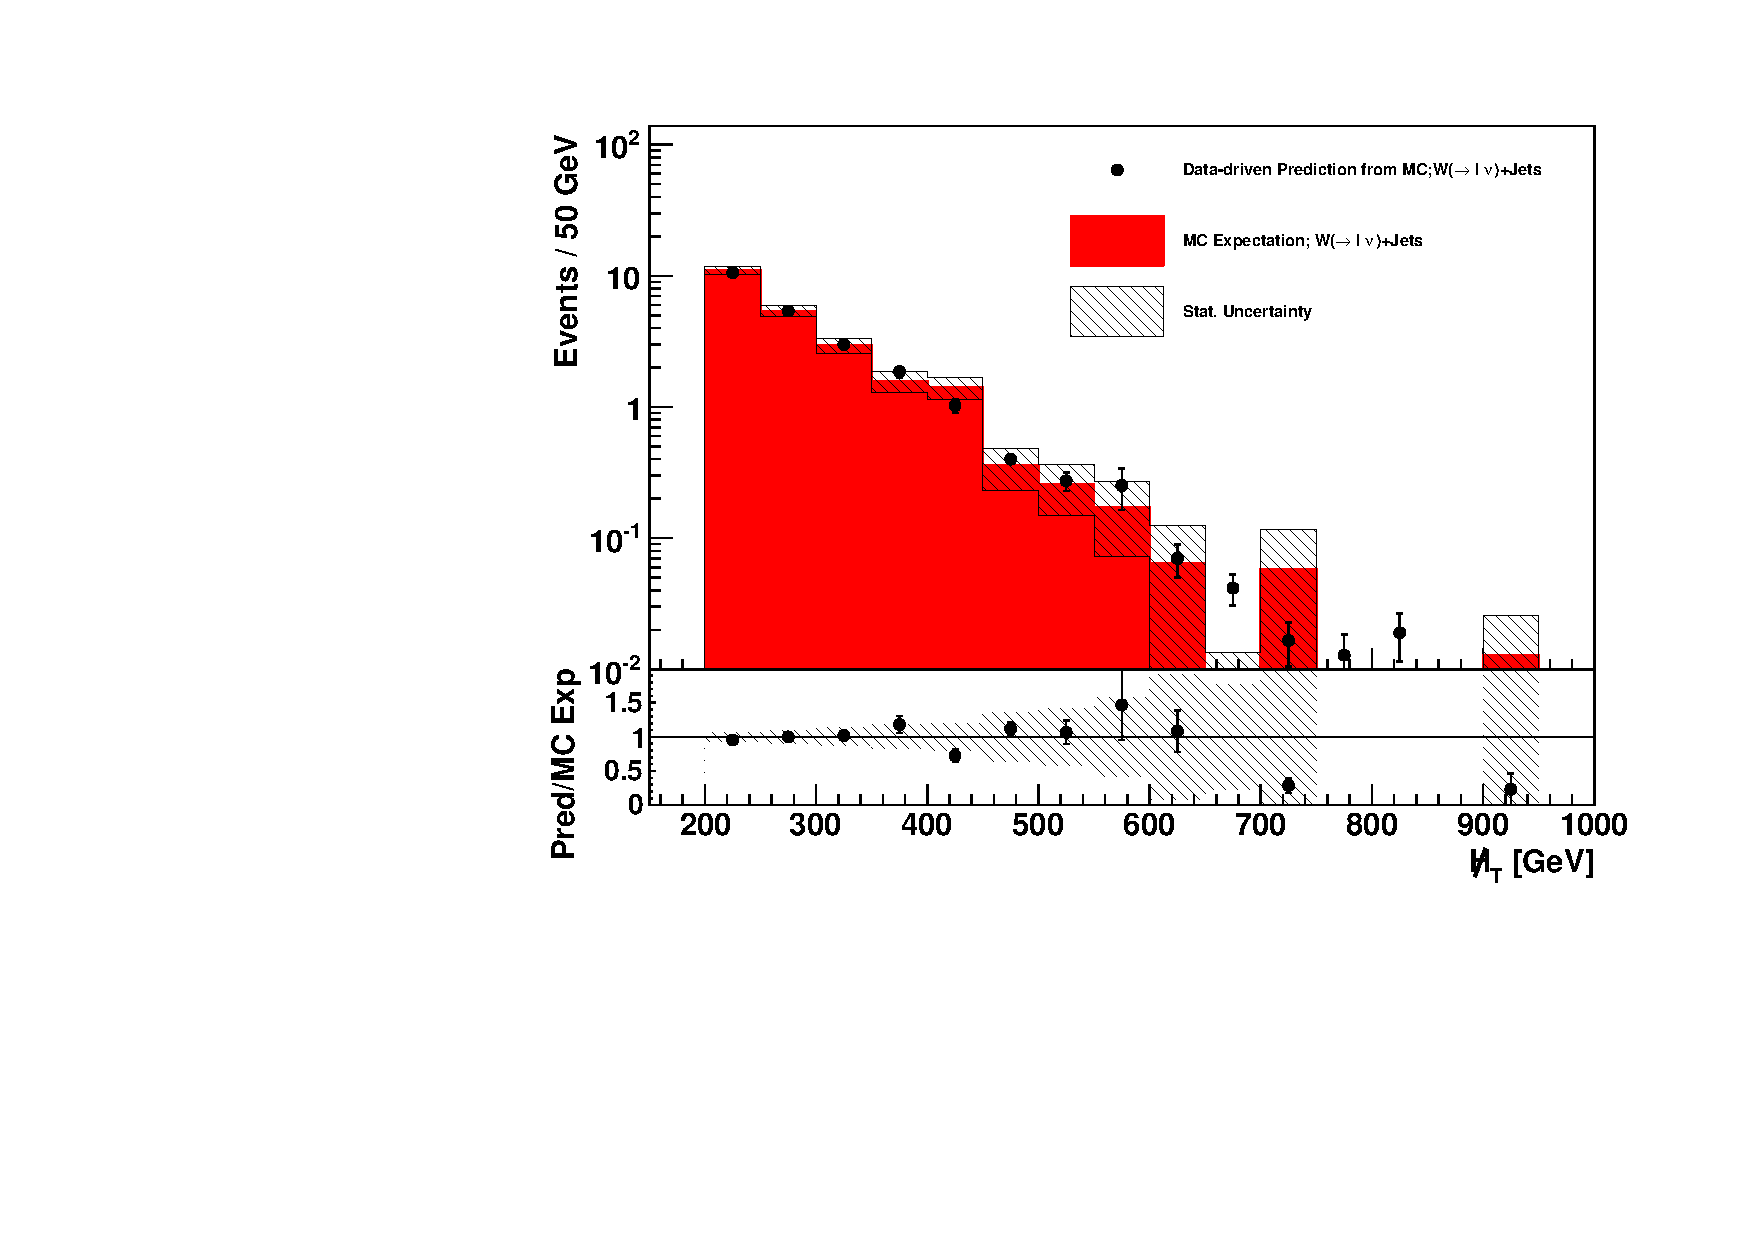
\includegraphics[width=0.45\textwidth]{lostlepton/plots/closure/MHTwIsoE.pdf} \\
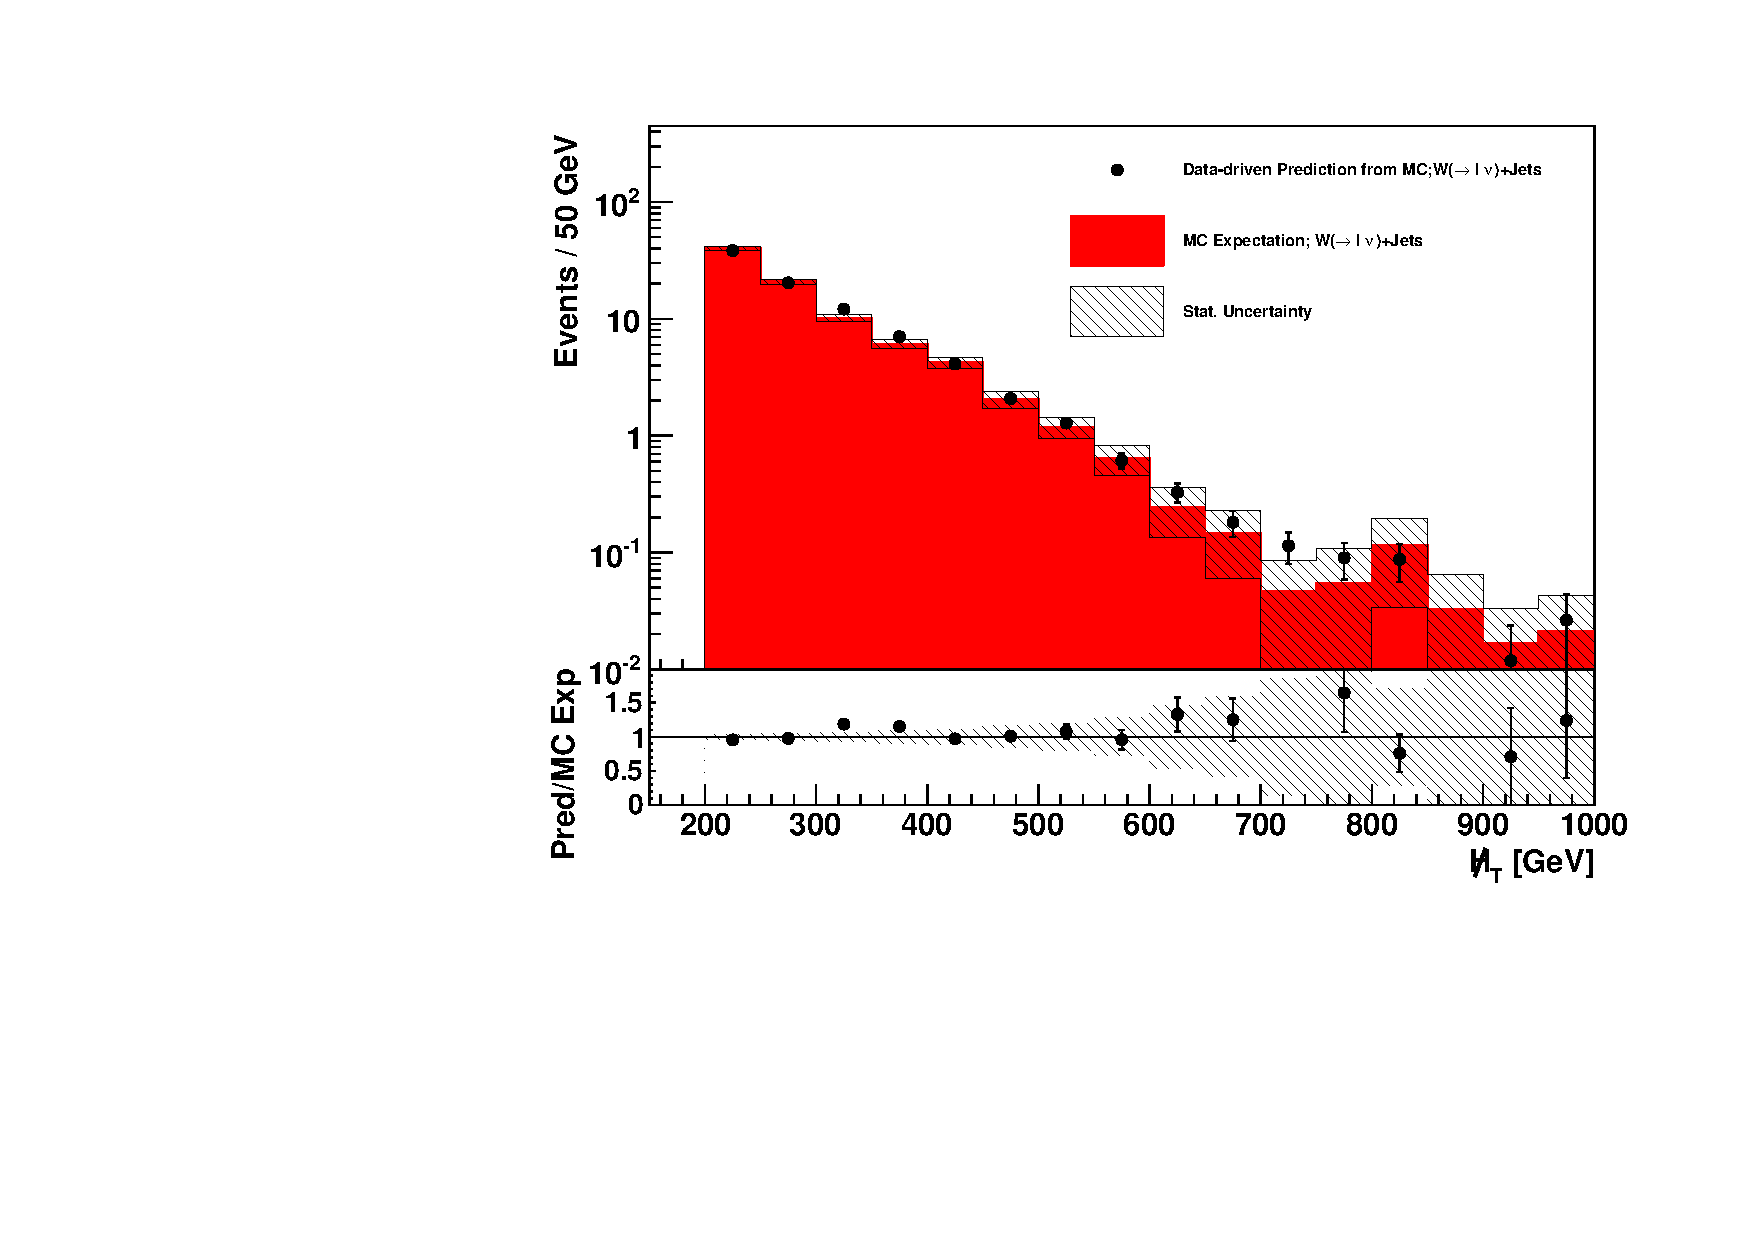
\includegraphics[width=0.45\textwidth]{lostlepton/plots/closure/MHTwRecoMu.pdf}
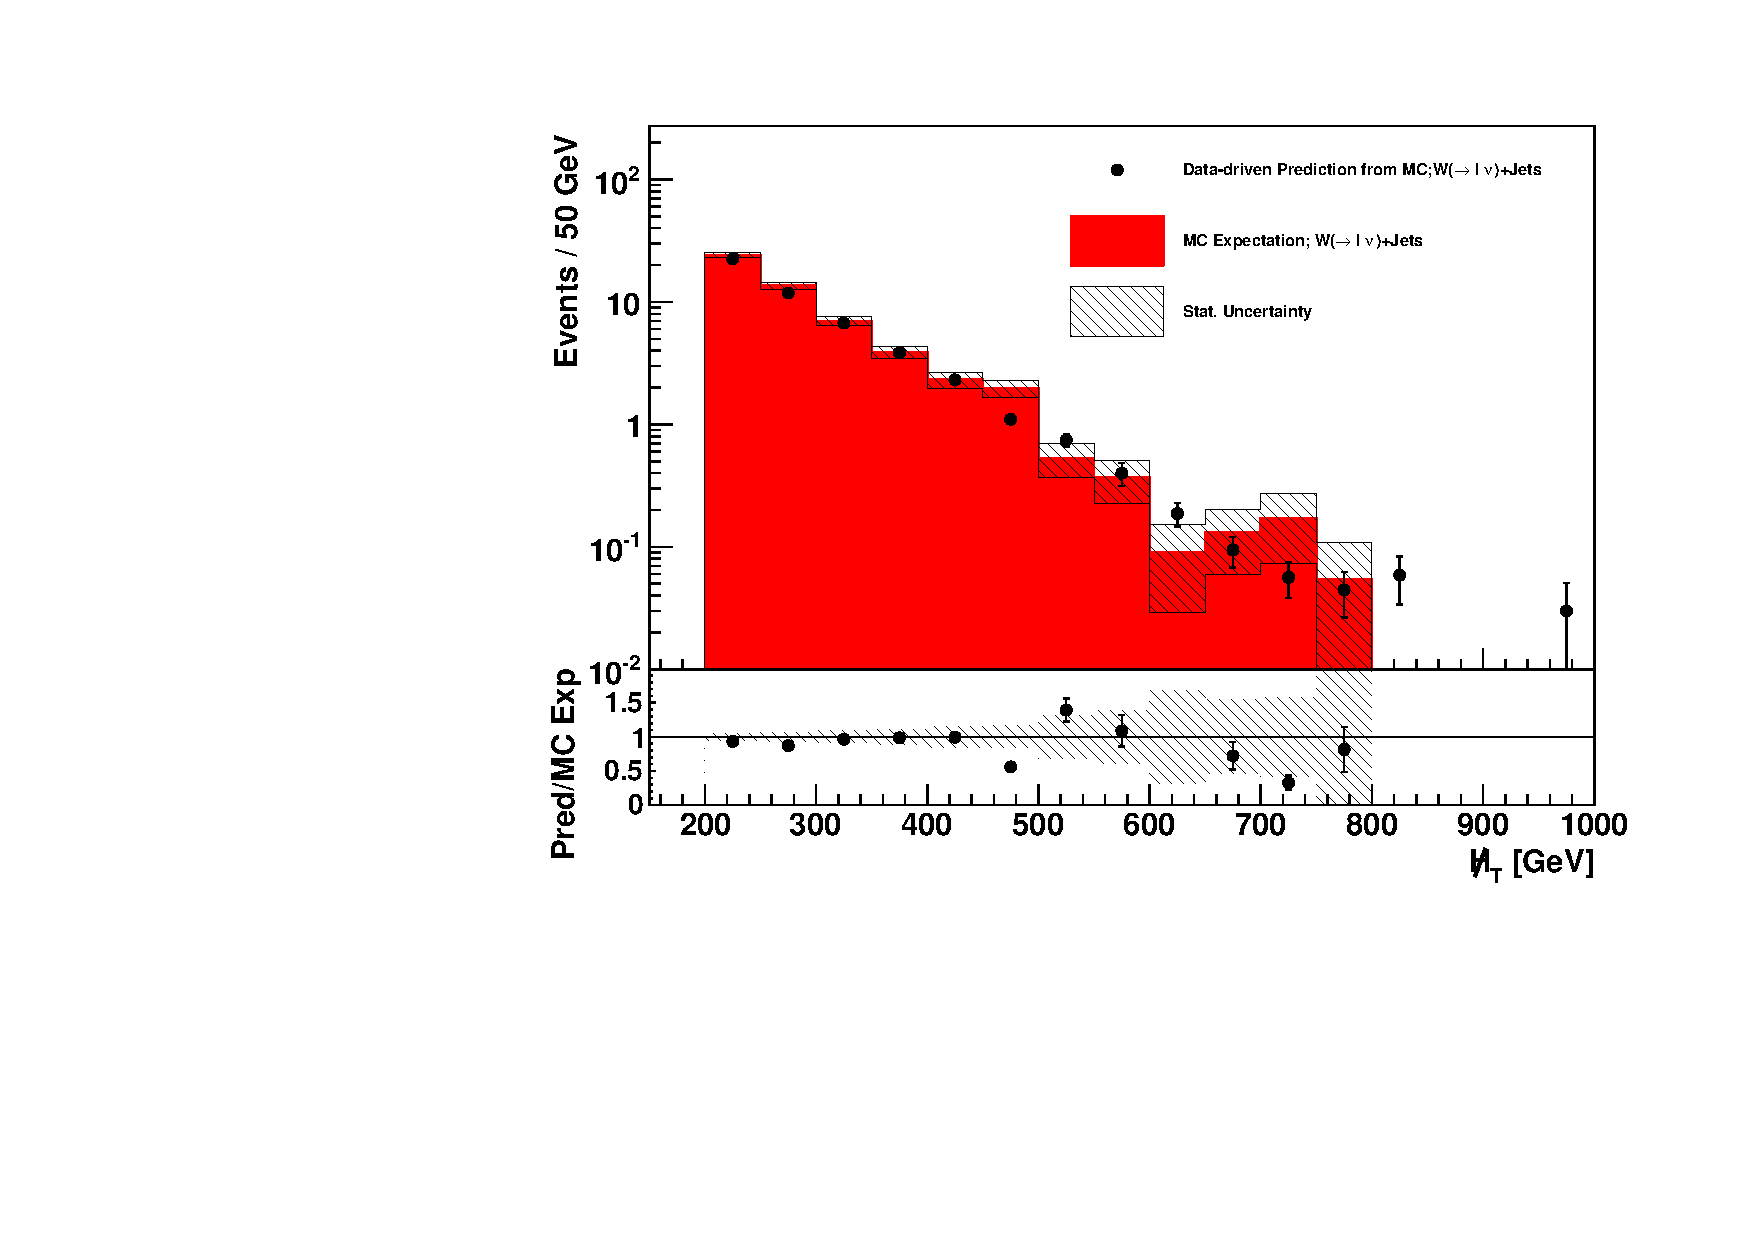
\includegraphics[width=0.45\textwidth]{lostlepton/plots/closure/MHTwRecoE.pdf}\\
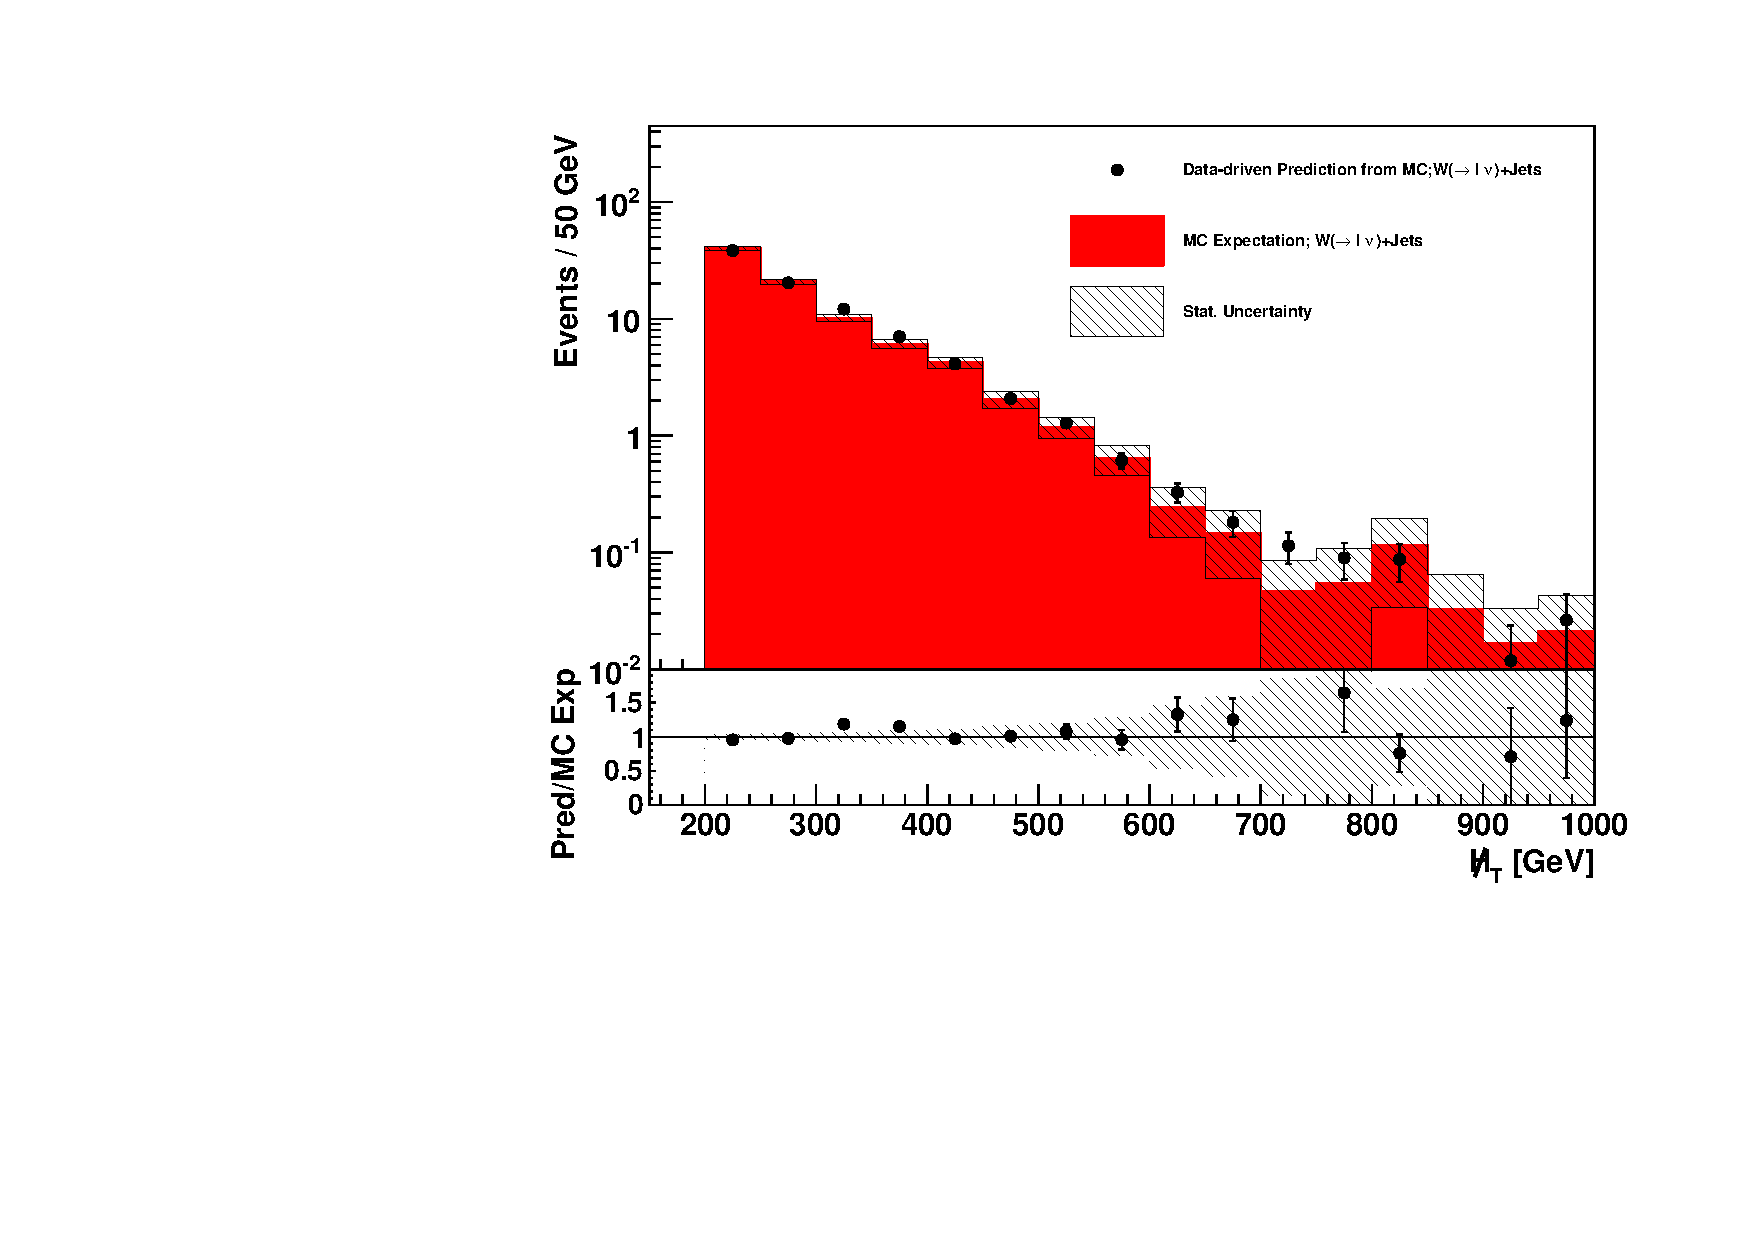
\includegraphics[width=0.45\textwidth]{lostlepton/plots/closure/MHTwAccMu.pdf}
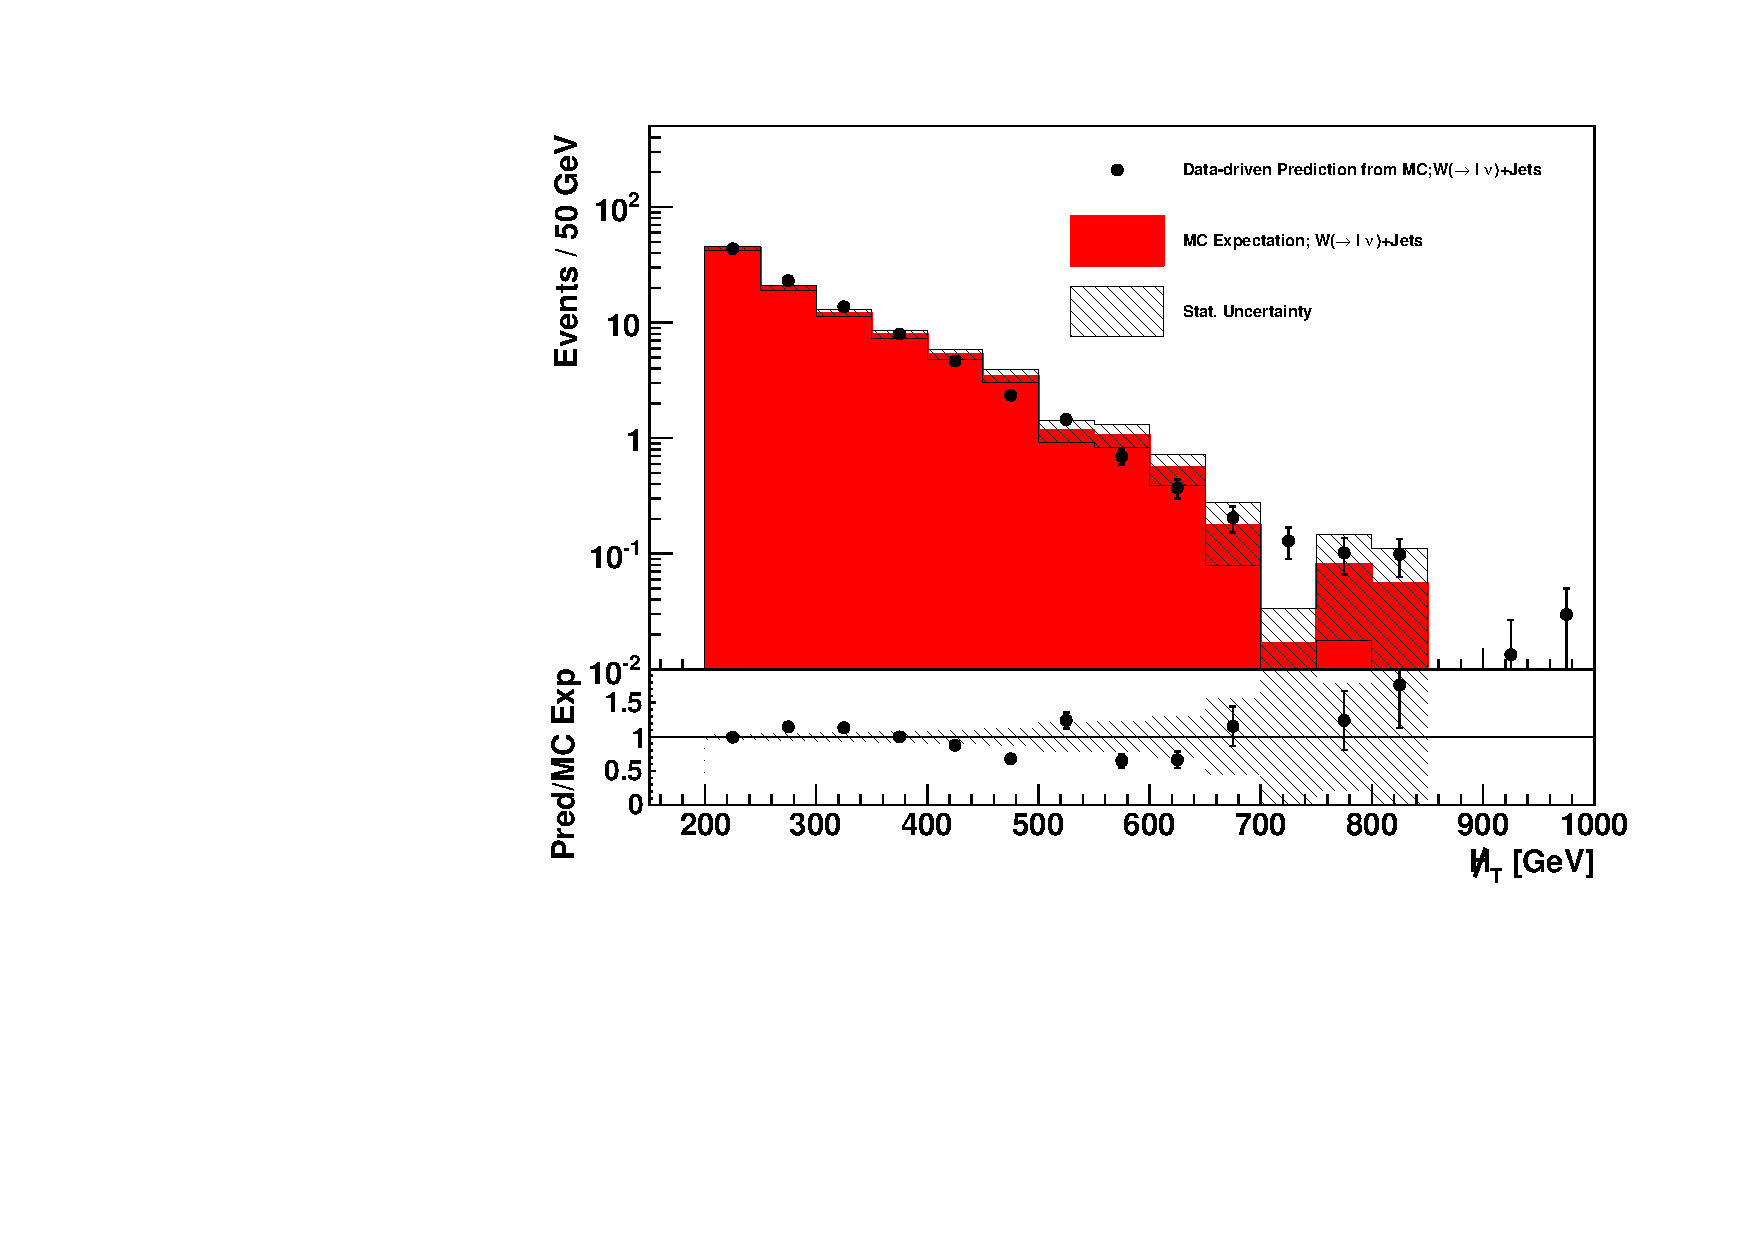
\includegraphics[width=0.45\textwidth]{lostlepton/plots/closure/MHTwAccE.pdf}\\
%\includegraphics[angle=0,width=0.5\textwidth]{wtop_lostlepton_figures/MHTMHT_r}&
%\includegraphics[angle=0,width=0.5\textwidth]{wtop_lostlepton_figures/HTHT_r}
%%(a)&(b)\\
\end{tabular}
\end{center}
\caption{This plots show the closure tests for \wpj separated for the not isolated (top), not reconstructed and out of acceptance fraction for muons (left) and electrons (right). Good agreement for the shape can be observed. The legend description can be found in the caption of Fig.~\ref{fig:closure_sepTTbar}.}
\label{fig:closure_w_sep_MHT}
\end{figure}

\begin{figure}[tbhn]
\begin{center}
\begin{tabular}{cc}
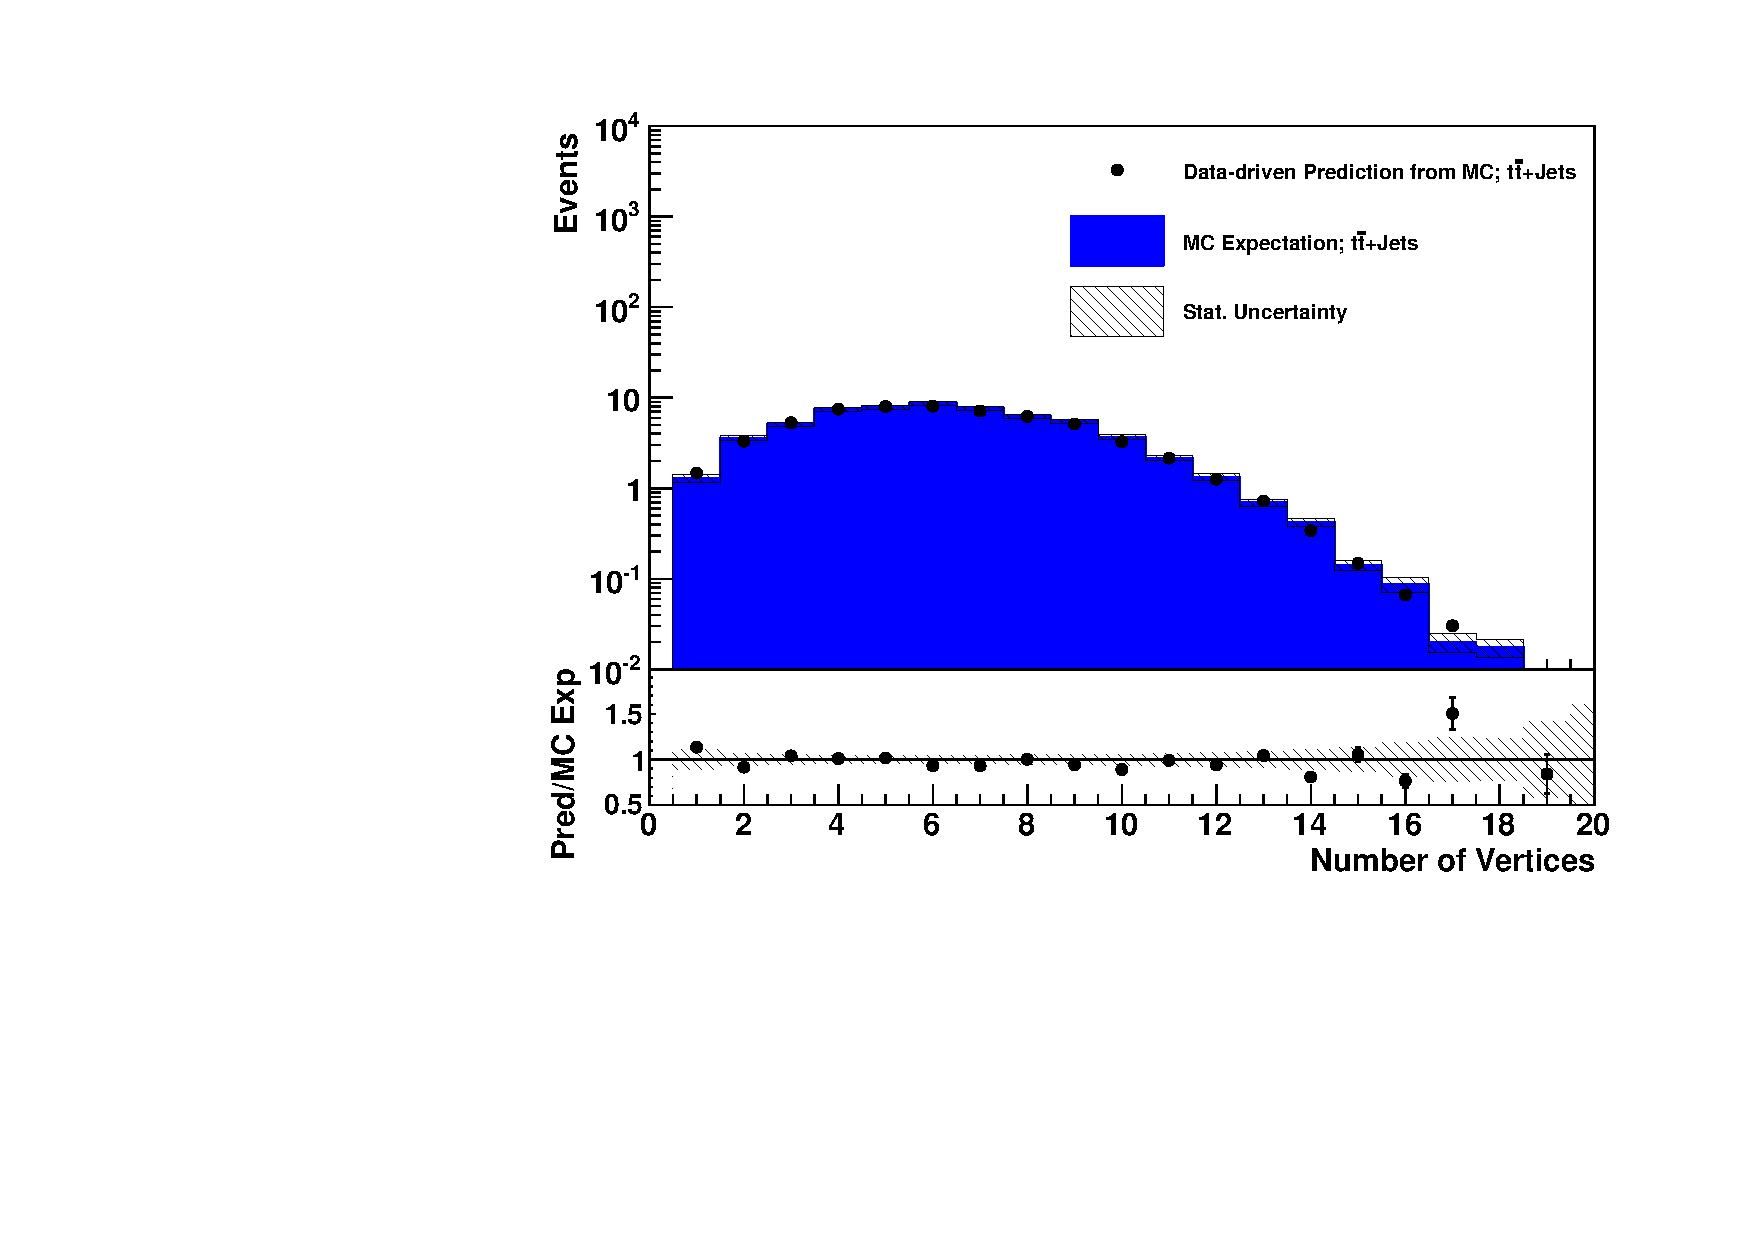
\includegraphics[width=0.90\textwidth]{lostlepton/plots/closure/NVttbarAcce.pdf}\\
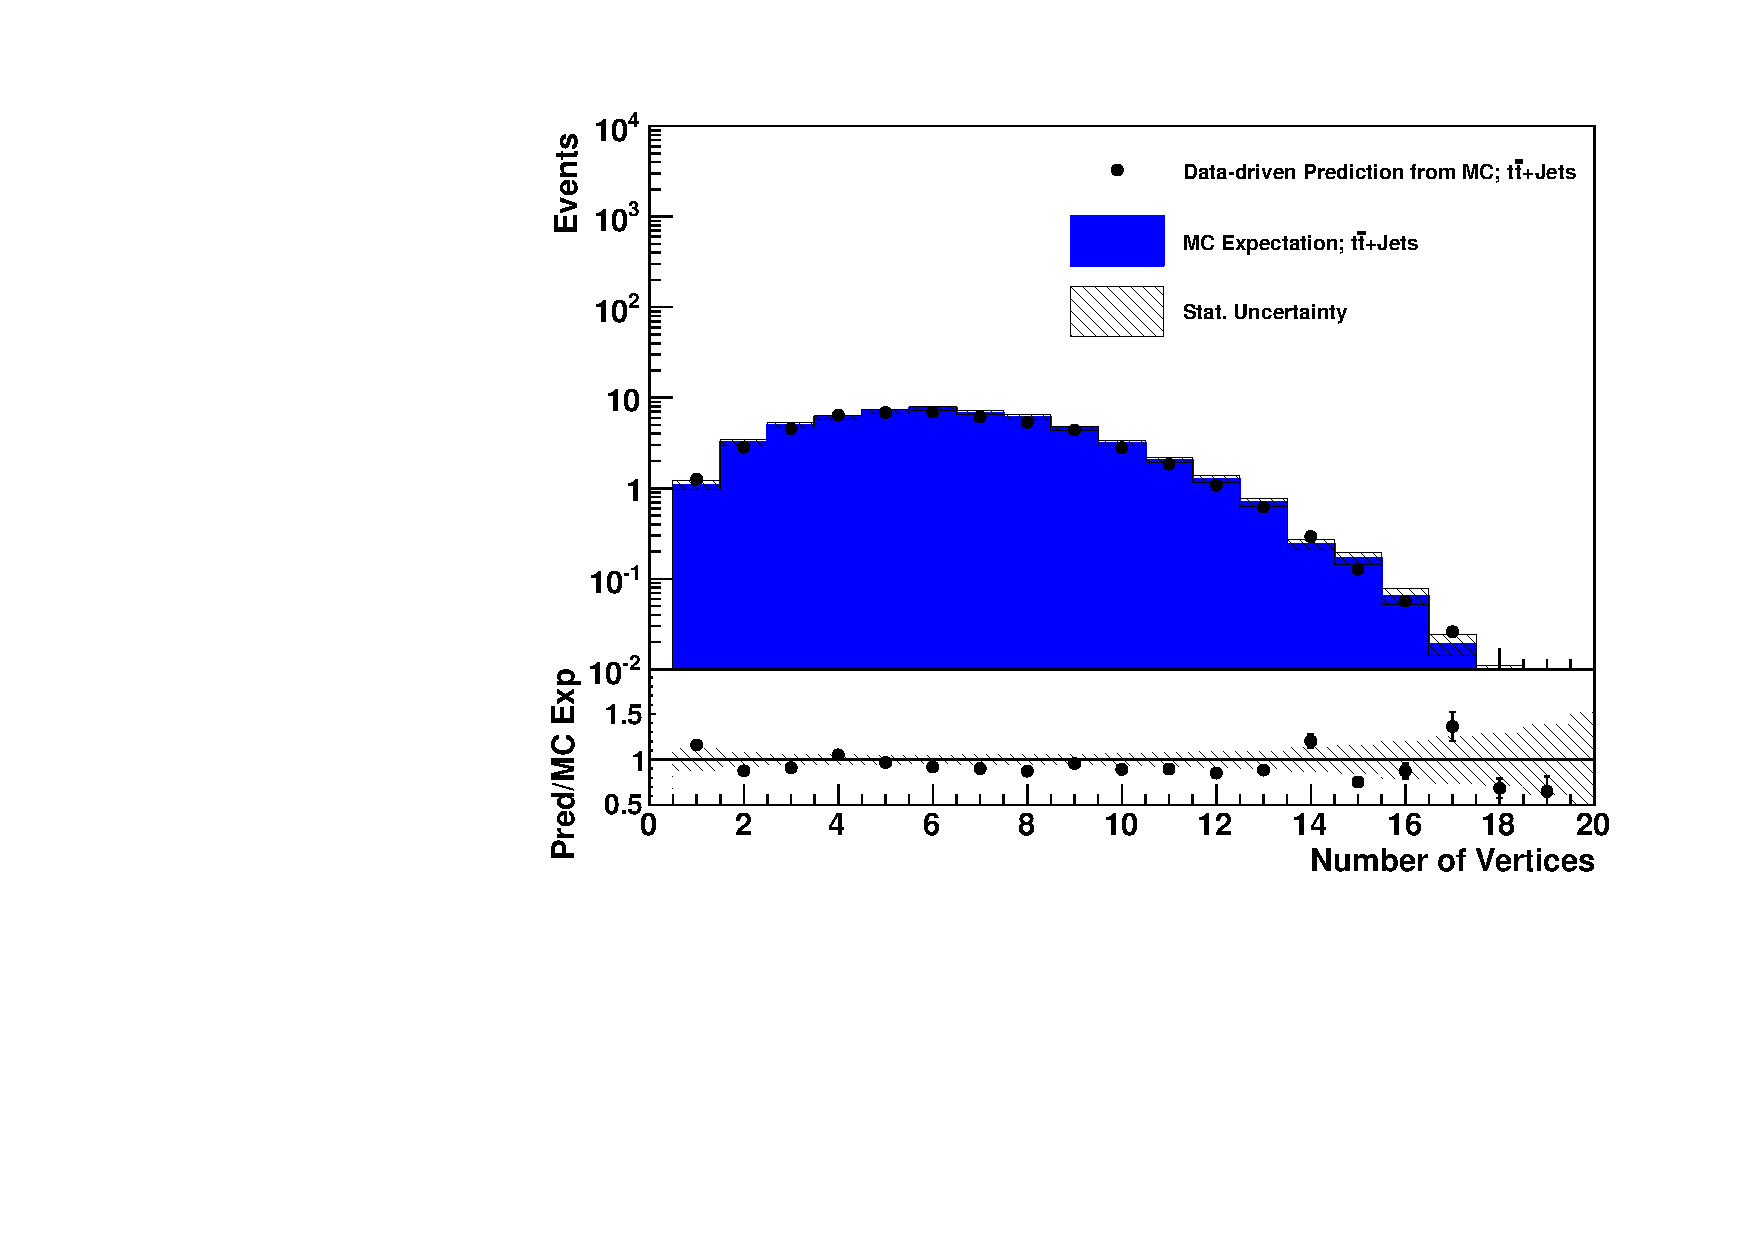
\includegraphics[width=0.90\textwidth]{lostlepton/plots/closure/NVttbarAccMu.pdf}
\end{tabular}
\end{center}
\caption{These plots show the closure tests for the out of acceptance electrons (top) and muons (bottom) for \ttbar, as the number of vertices. The legend description can be found in the caption of Fig.~\ref{fig:closure_sepTTbar}.}
\label{fig:pileup_acc}
\end{figure}

\cleardoublepage